Frames and components make up the external outlook of the device. Furthermore, it is the layer that allows the user to interact with the device. It consists of three subsystems which include laser and receptors, mister and speakers. 

\subsection{Laser and receptors}
This subsystem comprises of laser beams and receptors to detect the interference for the same. It consists of laser diodes pointed towards the photo resistors.  The receptors will not only detect the breaking of the beam, but also the number or note of the beam interfered. This information is then transferred to MIDI encoder for further analysis.

\begin{figure}[h!]
	\centering
 	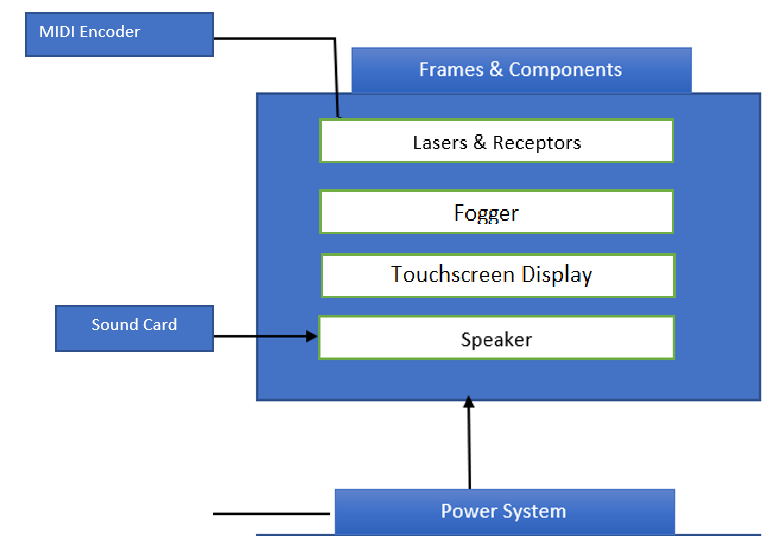
\includegraphics[width=0.60\textwidth]{images/Frame}
 \caption{Laser and Receptors subsystem description diagram}
\end{figure}

\subsubsection{Assumptions}
It is assumed that laser diodes are properly placed in position with respect to resistors. All the laser diodes are functioning properly, and no external factors are causing the interference other than the user.

\subsubsection{Responsibilities}
It is responsible for production of laser beams as well as recording of the breakage of laser beams. Furthermore, it should transmit those records to MIDI encoder.

\subsubsection{Subsystem Interfaces}
An external power supply is connected to the subsystem using breadboard or hookup wires. 

A USB to MIDI cable is used to connect the subsystem to encoder.

\begin {table}[H]
\caption {Subsystem interfaces} 
\begin{center}
    \begin{tabular}{ | p{1cm} | p{6cm} | p{3cm} | p{3cm} |}
    \hline
    ID & Description & Inputs & Outputs \\ \hline
    \#01 & Power supply & \pbox{3cm}{Electricity} & \pbox{3cm}{Power}  \\ \hline
    \#02 & MIDI Interface & \pbox{3cm}{Power Supply} & \pbox{3cm}{Laser beams}  \\ \hline
    \#03 & Receptors & \pbox{3cm}{Interference} & \pbox{3cm}{Event Messages/Signals}  \\ \hline
    \end{tabular}
\end{center}
\end{table}

\subsection{Mister}
It consists of an AGPtek aluminum mini mist maker which will be submerged into a water container in order to produce fog or mist which enhances the visibility of the lasers. Mister will take power source from an external outlet.

\begin{figure}[h!]
	\centering
 	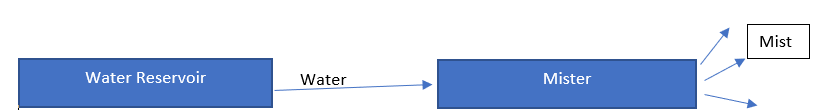
\includegraphics[width=0.60\textwidth]{images/Mister}
 \caption{Laser and Receptors subsystem description diagram}
\end{figure}

\subsubsection{Assumptions}
It is assumed that there is adequate water supply to submerge the mister. 

\subsubsection{Responsibilities}
It is responsible for emitting fog or mist which will be used to make the lasers visible to naked eye in well-lit room.

\subsubsection{Subsystem Interfaces}
Power is given to the mister through an external outlet.

Mister takes input from the water container which in turn converted into mist. 


\begin {table}[H]
\caption {Subsystem interfaces} 
\begin{center}
    \begin{tabular}{ | p{1cm} | p{6cm} | p{3cm} | p{3cm} |}
    \hline
    ID & Description & Inputs & Outputs \\ \hline
    \#01 & Mist Maker & \pbox{3cm}{Water} & \pbox{3cm}{Mist}  \\ \hline 
   \end{tabular}
\end{center}
\end{table}

\subsection{Speaker system}
It consists of single or multiple speakers which will be hooked up to the sound module. It will give the audio output for any presets or interference created by the user.

\begin{figure}[h!]
	\centering
 	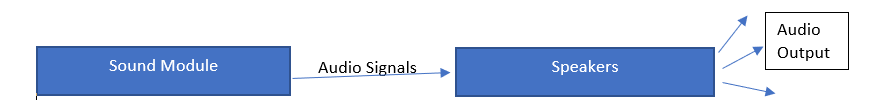
\includegraphics[width=0.60\textwidth]{images/Speaker}
 \caption{Laser and Receptors subsystem description diagram}
\end{figure}

\subsubsection{Assumptions}
Speakers are fairly new and the device is played in quiet place so as to ensure that there is no background noise.

\subsubsection{Responsibilities}
It is responsible for producing clear audio output.

\subsubsection{Subsystem Interfaces}
It receives the signals from the sound module and produces the resulting audio output based on the signals fed to it. 


\begin {table}[H]
\caption {Subsystem interfaces} 
\begin{center}
    \begin{tabular}{ | p{1cm} | p{6cm} | p{3cm} | p{3cm} |}
    \hline
    ID & Description & Inputs & Outputs \\ \hline
    \#01 & Speakers & \pbox{3cm}{Audio Signals} & \pbox{3cm}{Audio Output}  \\ \hline 
   \end{tabular}
\end{center}
\end{table}


